\documentclass[letterpaper,twocolumn,10pt]{article}

\usepackage{usenix,authblk}
\renewcommand\Affilfont{\itshape\small}
\usepackage{graphicx}
\usepackage{url}
\usepackage[toc,page]{appendix}

\makeatletter
\newcommand\appendix@section[1]{%
  \refstepcounter{section}%
  \orig@section*{Appendix \@Alph\c@section: #1}%
  \addcontentsline{toc}{section}{Appendix \@Alph\c@section: #1}%
}
\let\orig@section\section
\g@addto@macro\appendix{\let\section\appendix@section}
\makeatother

% Hi Everyone, we can start with this template Cynthia gave us and go from here
% The comment feature is great for annotating text, use it!
% pdflatex should compile this just fine for now

% This file will be the main file, I just splitted the sections in different latex files, so we can modify any section in an easy and simple way. I joined all the sections in the paper using the \input{filename} command.
\begin{document}

\title{Automated Election Auditing From DRE Logs}
\author[1]{P. Baxter}
\author[2]{A. Edmundson}
\author[3]{K. D. Ortiz}
\author[4]{A. M. Quevedo}
\author[5]{S. Rodr\'{i}guez}
\author[6]{C. Sturton}
\author[6]{D. Wagner}

\affil[1]{Clemson University}
\affil[2]{Cornell University}
\affil[3]{University of Puerto Rico-Arecibo}
\affil[4]{Miami Dade College}
\affil[5]{University of Puerto Rico-Mayag\"uez}
\affil[6]{University of California-Berkeley}

% Add additional authors:
% \and Author n
\maketitle

%Abstract

%Changes here (in the main paper I'll just invoke this file)
\subsection*{Abstract}
Voting audit logs, produced by electronic voting systems, contain information that is useful for uncovering procedural errors and election anomalies, but are currently unwieldy and hard for election officials to use in post-election audits.  We have devised a way to make the auditing process quick and efficient for election officials.  In order to audit elections, we develop new techniques for detecting equipment problems and procedural mistakes made by election workers; we have automated these analyses for a user-friendly process.  We implemented our methods and built a website for this tool that has the capability of analyzing electronic voting machine log files.  We intend for this work to assist those working with election auditing to quickly identify voting equipment or procedural issues and correct them before election results are certified.  Such issues include locating voting machines or media containing vote data that have not been included in the aggregated count, and voting equipment that needs maintenance before the next election.

%Introduction section
\bigvertspace
\section{Introduction}
\smvertspace
A DRE is a type of electronic voting machine in which the
voter interacts directly with the machine, typically through a touch
screen. DREs provide a friendly interface to assist the voter with the
ballot marking process. Similar to the commonly used optical scan
systems, DRE units can reduce overvoting and undervoting. Uniquely,
DRE machines can issue electronic ballots on demand; running out of
paper ballots is no longer an issue. Additionally, audio DREs can
assist visually impaired voters.
 
Federal standards require that electronic voting machines generate
detailed audit logs, which can be used during post-election
audits. These logs record events as they occur on the voting machine 
such as opening the machine for voting, casting a vote or closing the
machine at the end of election day. The log data may also include a
record of every ballot cast in the voting machine.  Previous work has
shown how these logs can be analyzed to uncover procedural errors and
anomalies that occur during the election\cite{Buell2011}.
Unfortunately, manual analysis of raw log data is usually cumbersome
and time consuming, making county-wide post-election analysis
impractical and prone to human error. Therefore, at the present time,
election officials do not regularly perform these types of analyses. 

We aim to make DRE audit log analysis more useful and accessible to
both election officials and other interested parties. In this work, we
develop new methods to analyze these audit logs for the detection of
both procedural errors and system deficiencies. We created a public
web application that applies our methods to detect procedural errors
and system deficiencies.  Election officials can use our tool to
identify memory cartridges containing precinct totals that were not
uploaded on election night, machines that may have experienced
hardware problems during the election, and polling locations that
closed late or had voters waiting in line for extended periods.
 
Our research builds on a similar study that was conducted with DRE audit data collected by fourteen South Carolina counties during the 2010 primary and general elections.  The authors of that study were able to determine, solely by analyzing the audit logs, that 1127 votes did not get included in the official certified tally in Richland County, South Carolina~\cite{Buell2011}. These findings were possible because DRE systems used in South Carolina produce three different types of audit logs, each capturing slightly different information. By cross checking the logs against each other, the authors found inconsistencies that enabled them to uncover the missing votes. In our research we used the same data set as a basis for development of our software. First, we replicated the detection of votes not uploaded. We took this matter further and found fifteen memory devices containing votes that were not uploaded to the tabulation systems from seven counties during the 2010 General election. These memory devices tallied 2082 total votes. Without additional information we could not verify if alternate procedures were used to add these missing votes to the aggregated totals. 

We implement these methods for the ES\&S iVotronic DRE as the 2010 South
Carolina data was already publically available through a previous
Freedom of Information Act request and the iVotronic was used in that election. \cks{Is this true? I changed the wording, but I'm not actually sure
  how the data was made available.} The iVotronic system is a
standalone, portable, touchscreen system that records vote totals,
ballot images and an event log on internal flash 
memory. The event log records, in chronological order, the system
events including unit configuration, polls opened, votes cast, polls
closed, calibration or battery issues, and system errors or warnings. 
iVotronic voting machines represent one of the most widely deployed
DREs in the U.S. In 2010, 422 jurisdictions tallying more than 22
million registered voters used this system~\cite{VerVot2010}. However, our methods for analysis of audit logs
are applicable to all DRE voting systems  that produce the necessary
audit logs.  

A brief description of several problems we detect follows.

\textbf{Votes not uploaded.} We detect  memory cartridges used to close voting machines that have not had their vote data uploaded to the tabulation system. This situation, if not corrected, can result in votes left out of the official results.

\textbf{Machines not closed.} We detect voting machines that were not
closed for voting at the polling location. Failure to close a machine
on election night may result in its votes being left out of the
certified count.

\textbf{Missing terminals from the audit database.} This analysis
identifies voting machines used during the election whose event log or
ballot images have not been uploaded to the election reporting
software. Complete DRE ballot images and event logs will allow for
more accurate post-election audits. 

\textbf{Polling location related analyses.} Our tool provides a series of analyses related to polling location activity. We identify locations that stayed open late as well as locations that may have experienced long lines during the day. This information can help county officials to identify locations that may need additional resources in the future. 

\textbf{DRE voting machine configuration and hardware problems.} Our tool performs several analyses that can identify  voting machines that may need testing, repair or reconfiguration. These analyses include identifying possible calibration issues, machines with potential power supply issues, machines that were forced to close early, and machines with incorrect date and time settings.

\textbf{Poll worker training related issues.} We also identify incorrect procedures at the precincts such as using the wrong cartridge to close the voting machines in a precinct, forgetting to print the precinct's zero tape or activating ballots with the incorrect cartridge. Election officials may be able to use this information to improve poll worker training and minimize recurrences in the future.

In this work we assume that DRE audit logs are complete, accurate,  trustworthy, and free of accidental or malicious tampering. Detecting and preventing audit log tampering is outside of the scope of this work.

In summary, this paper develops and implements new ways that audit log data can be used meaningfully and in an automated fashion to enhance the accuracy and efficiency of elections. We believe our tool will provide useful feedback to election administrators during the canvassing process. We hope that this study illustrates the potential value of voting systems' audit logs and motivates future election technologies to provide enhanced support for these purposes.




%Background section
\section{Background}

\subsection{Introduction to the iVotronic}
Approximately 422 jurisdictions in the United States used the ES\&S iVotronic electronic voting terminal in 2010.  A brief description of  its functionality and main system components follows:

\begin{itemize} 
\item Voting terminal. The voting terminal is a stand-alone touchscreen voting  unit. The ports available in the back of the terminal include: serial port, compact flash card slot and power supply port. The terminal is equipped with an internal battery which keeps the terminal operational during power failure periods. To comply with federal standards, at least one audio (ADA) terminal is placed in each precinct to assist the visually impaired voters.

\item Personalized Electronic Ballot (PEB). The PEB is a proprietary cartridge designed by ES\&S to operate the iVotronic terminal.  The PEB is placed in a slot located to the left of iVotronic\textquoteright s touchscreen. The terminal and the PEB communicate through the infrared port. The South Carolina counties deploy two types of PEBs to the precinct: a) the green band master PEB and b) the red band activator PEB. Both types of PEB have the same functionality, however, poll workers are trained to perform the following tasks with each PEB type.
    \begin{itemize}
    \item Master PEB.  Poll workers use the master PEB to open polls on election day. When the PEB is placed in the terminal, the touchscreen displays the precinct\textquoteright s name programmed in the PEB so that poll workers can verify the polling location information and date/time registered in the terminal\textquoteright s internal clock. If the information displayed is correct, the poll workers open the terminal for voting. The same master PEB should be used to open all terminals of the polling location. In the same fashion, the master PEB should be used to close all terminals of the polling location at the end of the voting day. When the terminal closes, it uploads  its totals onto the master PEB. The master PEB accumulates the precinct totals which are accumulated into the official tally.
    \item Activator PEB.  This PEB is used by  poll workers to activate ballots for voters. The number of activator PEBs that the election officials program for each precinct is proportional to the number of terminals and poll workers assigned to the precinct. The ratio varies depending on the jurisdiction criteria.
    \end{itemize}
\item Removable Compact Flash card (CF). The CF cards are programmed at election central and installed in the back of the voting terminal prior to precinct deployment. The CF cards contains graphic (bitmap) files read by the voting terminal during the voting process. The CF cards are also used as an external memory device: the audit log and ballot images are written to the CF card when the terminal is closed for voting. Once the polls close, the CF cards are removed from the back of the terminal and delivered to election headquarters on election night. 

\item External printer module. This module is connected to the serial port on the back of the voting terminal. The thermal printer produces the precinct zero tape and results tape. Poll workers are instructed to print the zero tape once all iVotronics of the precinct are opened for voting. In the same fashion, the results tape should be produced when all voting terminals are closed for voting on election night.
\end{itemize}

\subsection{Description of logs}
We used three iVotronic system logs to perform the analyses described in the next section. The event log (EL152.lst), ballot image file (EL155.lst) and the ES\&S election reporting manager system log (EL168a.lst).  The header of the log files identify the County's name, the type and date of the election, the date the report was generated and the election ID. The election ID is a parameter generated by the ES\&S election programming software to uniquely identify the specific election.

The event log (152.lst) lists all iVotronic terminals used on the election. The log records the terminal configuration at headquarters prior to precinct deployment which begins with the \textquotedblleft clear and test\textquotedblright of the terminal to delete previous election data from the terminal\textquoteright s memory. The log also records, in a chronological order, all relevant election day events including polls open and polls closing and the number of ballots cast.  The event log contains several columns which include: iVotronic's terminal serial number, PEB serial number, PEB type, date, time, event code and event description. An excerpt of  an event log is given in the appendix~\ref{app:el}.

The ballot image file (155.lst) contains all ballot images saved by the iVotronic terminals during the voting process. The ballot images are segregated by precinct and terminal where the votes were cast. The ballots are saved in a random order to protect the privacy of the voter. An asterisk (*) indicates the beginning of each ballot. An excerpt of a ballot image file is given in the appendix~\ref{app:bi}.

The system log listing file (EL168a.lst) tracks activity in the election reporting database since its creation at the election headquarters. Its chronological entries reflect the commands executed by the operator(s) during  pre-election testing, election night reporting and post-election canvassing. This log contains the totals accumulated in the various precincts during election night reporting, as well as any warnings or errors reported by the reporting software system during the tabulation process. The system log also tracks the uploading of the PEBs and CF cards to the central election reporting database. Manual adjustment of precinct totals are also documented in the system log file. An excerpt of a system log file is given in the appendix~\ref{app:sl}.

%Analyses section
\section{Analyses}
This section presents a description of our analyses and important findings.
\subsection{Votes Possibly Not Uploaded}
\subsubsection{PEBs Not Uploaded}
This analysis is intended to address the current Election Reprting Manager unavailability of reporting  a list of iVotronic machines or master PEBs assigned to each precinct. Currently, the election officials performing the vote tabulation on election night do not have a way to effectively compare the list of PEBs that have been successfully uploaded to the tabulation software with the pool of PEBs containing vote data throughout the county. This can lead to inaccuracies in election results if any PEBs containing vote data are accidentally left out of the tally process. Our tool provides an analysis that generates a list of PEBs used to collect votes on election day. It warns election officials of any PEB, master or non-master, that was used to close a terminal, whose data had not been uploaded to the election reporting system.   

Counties deploy two types of PEBs to each precinct on election day: a master PEB to open and close terminals and activator PEBs to issue ballots once the iVotronic terminals are opened for voting. The precinct procedures for poll workers dictate that a single PEB should be used to open and close all machines at a polling location. Failure to strictly follow this protocol led to problems in Miami-Dade County during the 2002 Primary election~\cite{Mazella2002}. In that case, poll workers used two or more PEBs to open and close terminals at their precinct.  However, election workers at county headquarters only uploaded one of these PEBs, expecting all machines to be closed with the same PEB. As a result, the votes from some machines were not collected on election night.  Election officials were forced to spend several days at the warehouse collecting all PEBs used in the election, printing tapes of every PEB, and uploading the votes from the PEBs that were not transported to election headquarters on election night. This caused a significant delay in the reporting of election results. A recent study found similar problems in several South Carolina counties~\cite{Buell2011}.

 This analysis is iVotronic specific. It requires the event log, the ballot image file, and the system log. The event log records the serial number of the PEB used to close the terminal.  It also records, in chronological oder, vote events processed in the voting machine. The system log file tracks a running log of the serial number of PEBs uploaded to the ERM tabulation system. The ballot image file provides a list of terminals used in each precinct.

Our method keeps track of the serial number of the PEB used to close each voting machine. It also records the polling location each voting machine was assigned to as well as the total votes cast in each machine. Then,  it verifies that each PEB that was used to close voting machines is uploaded to the ERM vote tally. It reports any PEB containing vote data that has not be added to the cumulative count.  For each such PEB, our analysis reports the serial numbers of the terminals collected in the PEB, the number of votes processed in those terminals and the precinct's name and number. With this information, election officials can gather the missing PEBs and collect votes from terminals not included in the cumulative totals.

\subsubsection{Machines Not Closed}
There are two main pieces of the election system that need to be analyzed to determine if votes were left out of the count.  We have discussed the first essential piece: the PEB.  The second piece of the election system that must be taken into account is the voting machine itself.   We have devised a way to determine which machines have not been closed for voting.  If a machine is not closed, then a PEB has not collected this terminal's data; our algorithm will help detect this situation where some votes were not counted.  

This analysis uses the event log to provide a report; the event log should have the ability to record events marking the opening and closing of each voting machine.  We created a method that checks if a machine was closed, given it was also opened for voting.  Our analysis searches through the event log for machines that were opened; these machines are stored in a data structure.  Next, we check that every machine in the data structure also recorded an event representing its closure.  If there are any machines that have been opened and not closed, they are displayed to the election official.   

\subsection{Polling Location Related Analyses}
\subsubsection{Polling Locations That Closed Late}
The polling locations in South Carolina must be opened for voting from 7 am until 7 pm. However, the electors waiting in line after 7 pm should be allowed to vote~\cite{VotingInfo}. Therefore, polling locations may stay open late in order to accommodate those voters prior to closing the voting machines on election night.  If election officials knew which places were likely to experience long lines, they could deploy more equipment or personnel to those polling locations.  Our tool can assist them by providing information about long lines that occur in this election.  Officials can use this information to make predictions about where long lines might occur in future elections.  

This analysis gives election officials information about how many polling locations had to stay open late and for how long.  It uses two iVotronic log files, EL152 and EL155. It also uses the iVotronic time/date verification function described in section~\ref{an:date} to exclude any terminals whose time stamp is probably inaccurate.  

This analysis generates a histogram detailing the number of polling locations that stayed open after 7 pm grouped by 10 minute increments. This information can be useful to election officials as they can identify how many polling locations that closed late and develop a strategy to mitigate those circumstances in future elections. Assigning additional resources to those polling locations can address bottlenecks at the precinct resulting in a more expeditious voting process during in future elections.
\begin{table*}
    \begin{center}
    \begin{tabular}{| c | p{5cm} | p{4.5cm} |}
    \hline                   
    \# Precint & Possibly not long lines experienced (p-value \textless 10\%)&Possibly long lines experienced (p-value \textgreater 10\%)\\
    \hline
    26 Huger&9:00 a.m. - 10:00 a.m. &7:00 a.m. - 9:00 a.m.\\
            &12:00 p.m. - 1:00 p.m. &10:00 a.m. - 12:00 m.\\
            &4:00 p.m. - 5:00 p.m. &1:00 p.m. - 4:00 p.m.\\
            &6:00 p.m. - 7:00 p.m. &5:00 p.m. - 6:00 p.m.\\
    \hline
    10 Cordesville &7:00 a.m. - 8:00 a.m.&8:00 a.m. - 12:00 m.\\
                   &12:00 m. - 1:00 p.m.&1:00 p.m. - 7:00 p.m.\\
    \hline  
    24 Hilton Cross Rd &12:00 m. - 1:00 p.m. &7:00 a.m. - 12:00 m.\\
                       &5:00 p.m. - 6:00 p.m. &1:00 p.m. - 7:00 p.m.\\
    \hline
    22 Hanahan 3 &7:00 a.m. - 5:00 p.m. &5:00 p.m. - 6:00 p.m.\\
                 &6:00 p.m. - 7:00 p.m.&\\
    \hline
    20 Hanahan 1 &12:00 m. - 1:00 p.m. &7:00 a.m. - 12:00 m.\\
                 &2:00 p.m. - 3:00 p.m. &1:00 p.m. - 2:00 p.m.\\
                 &5:00 p.m. - 6:00 p.m. &3:00 p.m. - 5:00 p.m.\\
                 &                      &6:00 p.m. - 7:00 p.m.\\
    \hline
    \end{tabular}
    \end{center}
    \caption{Long Lines in Berkeley County}
    \label{tab:line}
\end{table*}
\subsubsection{Long Lines}
Election officials assign voting machines and polling location supplies based on the number of voters registered in each precinct.  However, voter turnout can vary and as a result, some polling locations may end up overstocked with equipment, supplies or poll workers while others may lack resources or personnel on election day. Monitoring all the polling places in a large county can be a daunting task. Often, election officials don't have any process in place to monitor polling location usage. South Carolina counties have experienced voting machine bottlenecks during the 2008 and 2010 elections~\cite{Kreitman2010, Slade2008, U2010}.  Those counties can benefit from a tool that can analyze DRE audit data to identify peak times at the precincts.  This analysis can infer a steady flow of voters from two iVotronic log files (EL152 and EL155) and produce a report detailing possibly busy timeframes. Such information will assist election officials with the planning of future elections.

Our tool focuses on lines of voters by detecting heavily used voting terminals. When there are consecutive ballots cast with no time delay in between, we are able to infer that there is a line of voters at the voting machines. 

Once our tool groups the iVotronic units by polling location, based on the information contained in the ballot images report (EL155), it determines that all the machines in the voting location were in use. This analysis also uses a function that finds polling locations which closed late in addition to a time/date verification function that invalidates and excludes voting machines with anomalous date/time settings as described in section~\ref{an:date}. The date and time of iVotronic terminals is set manually and subject to human error; therefore creating inaccuracy in the timing of the events identified by the audit log.  The time verification function is significant in determining which machines were heavily used at the precinct in a specific time period; therefore inferring the possibility of long lines at the precinct.

To infer long lines, we focused on the polling locations that stayed opened after 7 P.M. as we could conclude they were busy processing the voters standing in line at that time. Our analysis calculates the time between consecutive votes before 7 P.M.; we keep track of the time that these votes occurred and the time difference between votes.  For all of the consecutive votes after 7 P.M., we only store the time difference between votes.  This data is found per machine, which allows us to match it to its respective polling location.  Then, we organize the time differences into one-hour time windows starting at 7 A.M. until 7 P.M.; all of the after-7 P.M. data was grouped together.  Then, focusing on the polling locations that close very late, we use the two sample Kolmogorov-Smirnov test to determine whether the votes cast in a particular time window come from the same distribution as the after-7 P.M. votes.  The result of the statistical test returns two values; one of them is the p-value. A p-value less than 10\%, indicates the two samples are unlikely come from the same distribution, and therefore there probably weren't long lines.  Otherwise, a p-value higher than 10\% is consistent with the two samples coming from the same distribution, however, we can not make any concrete conclusions based on a high p-value, we can only note that it is possible there were long lines in that polling location.

%which is the probability that the two sample data have the same distribution.  This p-value helped us establish whether a polling location had long lines at a certain time window.  If the p-value is more than 10\% then we can infer that the polling location possibly had long lines in that time window.
%Fix this part (add a table precinct name, p-value is less than 10%, p-value > 10%), then explain the table.
Table~\ref{tab:line} summarizes the times periods when the Berkeley County polling locations experienced long lines before 7 p.m. We found that 17 precincts were closed after 7:30 P.M. and decided to run the analysis in these locations to determine when there were long lines.  We will emphasize the top five precincts that close very late.  Our analysis reveals that the first precinct Huger \#26, which closed at 8:43:44 P.M., has higher p-values at 7:00 A.M., 8:00 A.M., 10:00 A.M., 11:00 A.M., 1:00 P.M., 2:00 P.M., 3:00 P.M. and 5:00 P.M..  The minimum p-value is 15.4\% at 2:00 P.M. and the maximum is 66.0\% at 11:00 A.M.  Precinct Cordesville \#10 could possibly have had long lines throughout almost the entire day, except for 7:00 A.M. and 12:00 P.M. with a minimum p-value of 13.6\% at 10:00 A.M. and the rest of the time had p-values higher than 20\%.  Precincts Hilton Cross Rd \#24, and Hanahan 1 \#20 also had long lines almost all day.  Precinct Hanahan 3 \#22 only experienced long lines at 5:00 P.M. with a p-value of 38.5\%.  We can conclude that these precincts have experienced long lines during the whole day and it may be the reason for which those precincts closed very late.

We strongly recommend election officials to conduct this analysis after each election to plan for future elections of the same type. Assigning additional personnel, whether poll workers or rovers, and machines to the busy polling locations may reduce long lines of voters.  Our analysis can detect when there is a steady flow of voters, but it does not determine if the long line of voters is caused by a slow registration process or too few voting machines.


\subsection{Hardware Issues}
Election officials may be interested in identifying machines that have hardware problems, such as screen calibration issues, machines with a low battery, terminals that closed early, and machines that recorded unknown, but possibly severe events.  The first of these analyses detects machines with recurring calibration errors and machines that had recorded votes while possibly not calibrated.  By finding the events that correspond to a screen that is not calibrated and to the recalibration of that screen, we can find if votes were cast in between those times.  The second analysis regarding hardware issues looks for machines with an unusually large number of events titled \textquotedblleft Terminal shutdown - IPS Exit\textquotedblright .  We infer that these machines have a low battery because they experience a more-than-normal number of events related to the Internal Power Supply.  Additionally, our tool searches for machines that recorded a warning event about the terminal closing early.  In order for this event to occur, a trained technician must enter a password to access the service menu and make a particular selection to close the machine.  If a machine is closed in this manner during election day, there must be something wrong with it that is preventing votes from being cast correctly.  Lastly, there is a set of events that have questionable meanings, but could potentially represent hardware issues.  

Analyses such as these can help officials identify machines that may require maintenance or to be replaced.  In the case of a machine having ballots cast on it when it is not calibrated, it may not have captured the voter's intent.  Depending on the magnitude of the situation, this could cause a different outcome in the election.  If our analyses detect other hardware problems with a machine, it may not be recording votes accurately; these votes may not even appear in the event log or ballot images.  If the event log and the ballot images do not record ballots being cast, then it is nearly impossible for officials to realize votes are not being counted.  

Due to the available resources and the nature of these analyses, assumptions were made regarding the meaning of events and the severity of the situation.  Currently, there is no user manual or detailed description of the events that appear in the event log; because of this, we are not able to guarantee that the event \textquotedblleft Terminal shutdown - IPS Exit\textquotedblright means the machine has a low battery.  This assumption is also applicable to our calibration analysis and our detection of unknown warning events.  If a description of each event was available, we could be more definitive in our results and possibly implement analyses that report other useful hardware failures.    

[Statistics from reports here] [Suggestions/corrective actions to take].

\subsection{Procedural Errors}
Our tool can detect procedural errors and poll worker mistakes; a few of these are: precincts that do not print zero tapes on the morning of election day, using a master PEB to activate ballots, opening and closing machines with different PEB.  According to the South Carolina poll worker training video (citation), poll workers are required to print at least one zero tape per polling location on the morning of the election.  Using the event log, our tool checks each polling location for this event and reports the locations that did not record this event.  Another way our tool finds procedural errors is by crosschecking the master PEBs with the PEBs used to activate ballots.  Poll workers should be using non-master PEBs to activate ballots so that the PEBs do not get switched.  Along the same lines, we report incidents of opening and closing a machine with different PEBs.  A machine should be opened and closed with the same master PEB; if not, it may be more likely that this PEB does not get uploaded.   When poll workers cancel ballots, they must select a reason why; this is another way to detect errors.  There are seven options for canceling a ballot: wrong ballot, voter left after the ballot was issued, voter left before the ballot was issued, voter request, printer problem, terminal problem, or an unspecified reason.  If there are any instances of canceling a ballot due to a printer problem, it could be an indicator of a procedural error because ballots are not printed.  In other cases, if there is a large number of a specific reason, such as having the wrong ballot, this could indicate the poll workers are repeatedly issuing the wrong ballot.  

It may be beneficial to election officials if they could detect which locations poll workers are following the required procedures in order to mitigate larger problems.  If election officials are aware of the procedures that are not being followed, they will hopefully be able to mitigate them.  This will allow for more efficient audits as well as a better voting experience for voters.  Procedural errors can cause many problems including lost votes, incorrect vote counts, disgruntled voters, and long lines.

While our analyses detect an important set of errors, there are certainly many more procedures that can be analyzed.  In addition to printing zero tapes in the morning, poll workers are required to print results tapes at the end of the election; unfortunately, this is not detectable due to the way the event log is produced.  We have inferred from the event logs that the poll workers are extracting the compact flashes before printing the results tapes, therefore the event log shows no record of the event.  

[Statistics from reports here] [Suggestions/corrective actions to take].

\subsection{Systematic Date and Time Errors}\label{an:date}
The iVotronic DREs append each audit event in chronological order.  Each event is marked with a time-stamp based on the DRE's internal clock.  We discovered and report on a variety of errors by classifying the type of errors experienced. Correct time-stamps are critical in post election audits and often incorrect stamps can not be automatically corrected post election.  Previous works identify and remark on some of these date errors~\cite{Buell2011,Sandler2007}.  We further attempt to classify and automate the identification of these issues.

Erroneous time-stamps can invalidate the audit-logs and often preclude data from being used in automated reports.  Determining machines to have either valid or invalid time-stamps has a lot of gray area and different errors will affect different analyses.  Some machines experienced time-stamps that would blank to \textquoteleft 00/00/00 00:00:00' for only a couple of events.  This naturally wouldn't affect data looking at opening and closing times, but would create outliers or gaps in data measuring time between votes cast.  

We found it simplest to classify date errors into two categories.  Those errors resulting from machines not having their clocks set appropriately and those resulting from apparent bugs in the iVotronic time-stamp mechanism itself.  Our website includes an automated a report that attempts to identify and group as many of these errors as possible.

First, machines shipped or set with incorrect dates were identified.  These errors all suggest the need for a more thorough pre-election check of each machine's clock.   Any machines experiencing manual clock adjustments on election day were included in the report as well as those machines which opened for voting on a date that was wildly incorrect (i.e. dates well before pre-election or dates after election day). This mostly included machines that did not account for Daylight Saving Time or  those machines that didn't set their initial date until after opening for voting.  All the above machines were checked as closing on a valid election day.  Pre-voting dates were not considered as they appeared to be inconsistent among the different counties. Machines which open and close on an improbable dates are separately identified as machines that had bad dates that went uncorrected..  

Machines experiencing additional date errors were classified in a separate report.  Many machines were found to have anomalous date changes that weren't paired with the normal date set event. [Figure 1 will show the 4/12 jump in Berkeley county] Often before the clock on a machine is first set the dates will show up as being many years into the future or as a zero date.  This isn't a problem as most  of these machines are set correctly before being opened for voting.  However, there are many places in the logs were the date will seemingly randomly jump to a date far into the future or the past and remain there until manually corrected.  [Figure 2 12\/21 in Berk County] shows a case where the date jumps ahead to 12/21/2010 for two events before changing back.  These machines were automatically identified by looking for any major date jumps that occur on election day or zero stamps being recorded after machines are open. Machines experiencing many date jumps may require troubleshooting from ES\&S.  It may be a more systematic issue that the date on an iVotronic can apparently change for no reason.

We strongly advise that procedures for setting the clocks on machines are reviewed.  The unknown date jumps seen in the logs are concerning, but generally are not creating as many audit issues compared to machines whose date were never set correctly.

Accurate clocks directly impact the usefulness and correctness of the audit logs. Ensuring that every single machine is set correctly is not necessarily a simple task.  We would recommend that each machine is configured accurately before being sent to the precincts.  Additionally, all machines should be double checked for a correct time before opening for voting.  Daylight Saving Time settings are also potential concern.  Many machines (statistic for anderson) were found to be adjusted forward by an hour during election day.  

The Authors of \textquotedblleft Casting Votes in the Auditorium\textquotedblright~\cite{Sandler2007} propose a distributed network between DREs.  This \textquoteleft Auditorium\textquoteright provides a far more robust system to ensure accurate and verifiable audit logs.  They propose a system where all the election machines are networked together and append to a common audit log verified by each machine.  This allows for more error redundancy and removes the logistical issue involved in making sure every single machine has their date correctly set.

% Related Work section
\section{Related Work}
Many election technology systems provide a means of auditing elections. For example, in optical scanning systems the cast ballots themselves form a paper record of the votes cast on election day. On the other hand, DRE machines do not provide this type of paper trail. Some DREs provide a Voter Verified Paper Audit Trail (VVPAT), which stores a hard copy version of each ballot cast.  A third type of audit trail, which is produced by all DREs, are the event logs stored electronically on each DRE.  In this section we discuss related work on the analysis of audit logs for post-election auditing. 

Two recent studies used event logs from the iVotronic voting system to audit elections~\cite{Buell2011,Sandler2007}. The authors of the first study~\cite{Buell2011} performed an audit of the same South Carolina elections that we analyzed. Using these audit logs, they discovered votes not included in the certified counts and problems with the audit data. They crosschecked the event log, the ballot images file, and the system log to identify unsupported votes and missing audit data.  By consulting additional audit materials, such as the printed results tapes, the authors were able to offer possible reasons and explanations as to why the problems occurred. Our work takes a slightly different approach.  We focus on developing a variety of methods to analyze the data; in addition, we automate these analyses in order for their use by election officials.  While our tool did discover and report these same problems, we simply report what was wrong, but can not provide a possible explanation for the cause of the error. 

The authors of the second study~\cite{Sandler2007} provided an analysis of vote tallies using the protected count of votes on each machine and comparing this to the printed results tapes. Their report also finds dates that were most likely inaccurate.  With further investigation, they concluded that the hardware clock was incorrect. Our research provides analyses to identify similar problems, but in a way that could be automated. 

There has also been research on using the audit logs to analyze election-day procedure and activity. For example, one recent publication showed how event logs could be used to determine if a machine acted \textquotedblleft normally\textquotedblright on election day~\cite{Antonyan2009}. The authors of this research studied the event logs of the AccuVote Optical Scanning system and used those logs to build a finite state machine that models the sequences of events a well-behaved machine might produce. This type of analysis would be useful to provide for the iVotronic systems that we studied. However, the AccuVote machines have considerably fewer possible event types than the iVotronics so the analysis would become considerably more complex. 

A common problem on election day, which we try to identify in our analysis, is the occurrence of long lines. Many studies have researched ways to mitigate long lines at polling locations ~\cite{Allen2006,Dow2007,Spencer2010,Wilson2008}.  One such study has simulated the flow of voters through the voting process~\cite{Edel2010}. The authors use this simulation to determine the optimal number of voters per voting machine, and correspondingly, the appropriate number of voting machines per polling location based on the number of registered voters at that particular location. Their work is predictive: the authors make some assumptions, such as the average time it takes to vote and when peak voting hours will occur, and use those as a basis for predicting where long lines are likely to occur. Our analysis is descriptive: given the audit logs from election day, we infer the average time it took to vote and use that information to determine whether a particular polling location experienced long lines or not. The two methods are complementary. Predictive models can be used to prevent long lines, while descriptive models can be used to check and refine the prediction algorithms. 

Voter Verified Paper Audit Trails (VVPATs) are a different type of audit log. Unlike the audit logs we used in our analyses, VVPATs are viewed and verified by the voter and are more suited to audits concerning a DRE incorrectly capturing a voter\textquoteright s intent. Our work is more concerned with identifying cases of cast votes not being included in the final count, or issues at the polling place that might prevent the voter from casting their vote in the first place. With VVPATs, as long as a certain percentage of voters do check their paper ballot~\cite{Hall2006}, the voting machine need not be assumed correct, whereas our analyses do make this assumption.

% Future Voting System Suggestions
\section{Future Voting System Suggestions}
[To complete by Wednesday].
%Conclusion
\section{Conclusion}
We recommend that election administrators conduct routine reviews of the audit logs generated by the voting machines as they contain useful information that can shed light on procedural and election equipment issues. This paper develops methods to analyze audit data from DRE voting machines intended to assist those working with election auditing and integrity.   We perform a variety of analyses on the DRE audit data to detect possible miscounts, procedural errors, voting machine malfunctions, or system deficiencies. With this information, election officials can improve poll worker training, election official checklists, election tabulation procedures, and voting machine preparation testing.

We built a web application to perform these analyses. Election officials just need to upload the DRE log files to our website and run the analyses. By automating our analyses we can provide intelligent feedback to election officials during the canvassing process and help them quickly correct any problems in order to produce accurate election results. These analyses are freely available online at www.audit-bear.org.

%Acknowledgements section
\section{Acknowledgments}


%This tells latex to use our .bib file
\bibliographystyle{plain}
{\footnotesize
\bibliography{paper}}

%Appendix section
\clearpage
\onecolumn
\begin{center}
\appendix
\section{Event Log File}\label{app:el} 
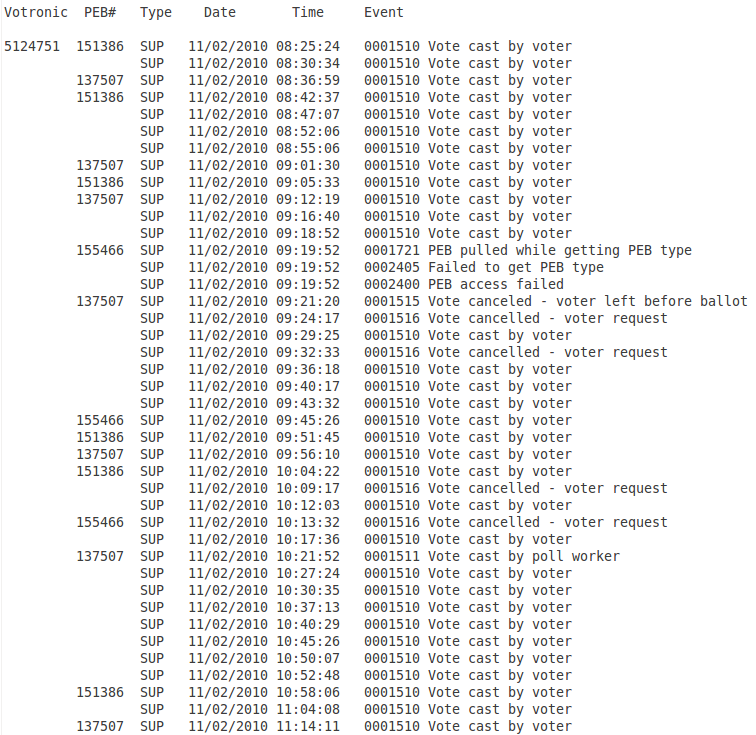
\includegraphics[width=0.8\textwidth]{eventLog}
%~\ref{app:el}

\clearpage
\section{Ballot Image File}\label{app:bi}
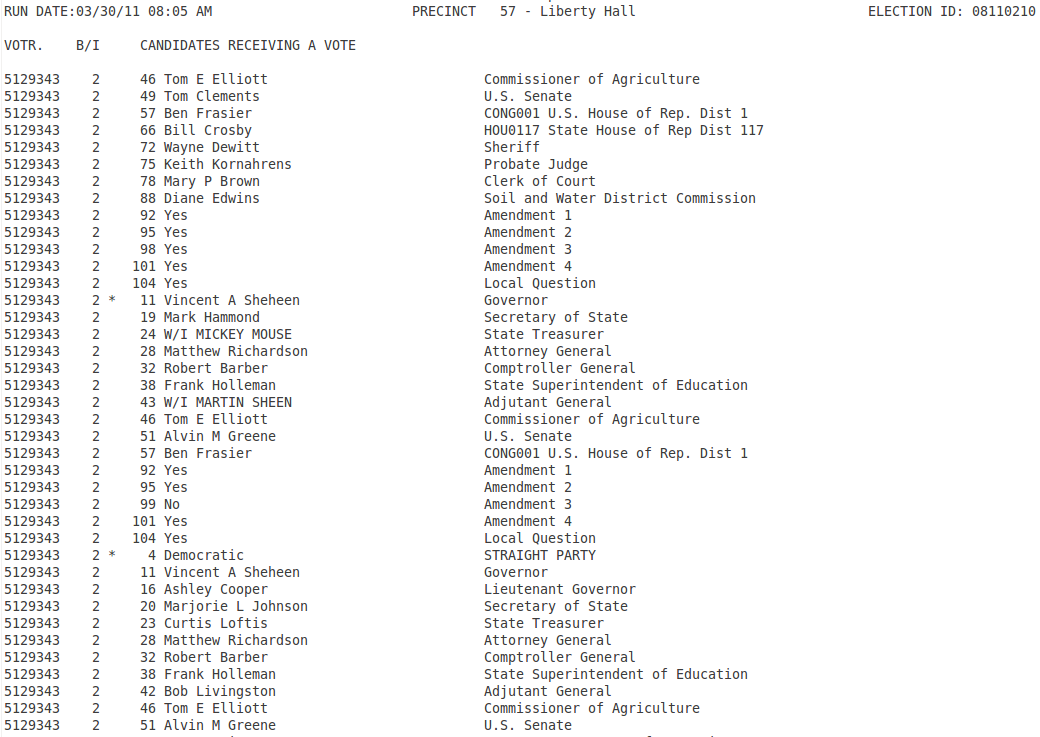
\includegraphics[width=0.9\textwidth]{ballot}
%This is app~\ref{app:bi}

\clearpage
\section{System Log File}\label{app:sl}
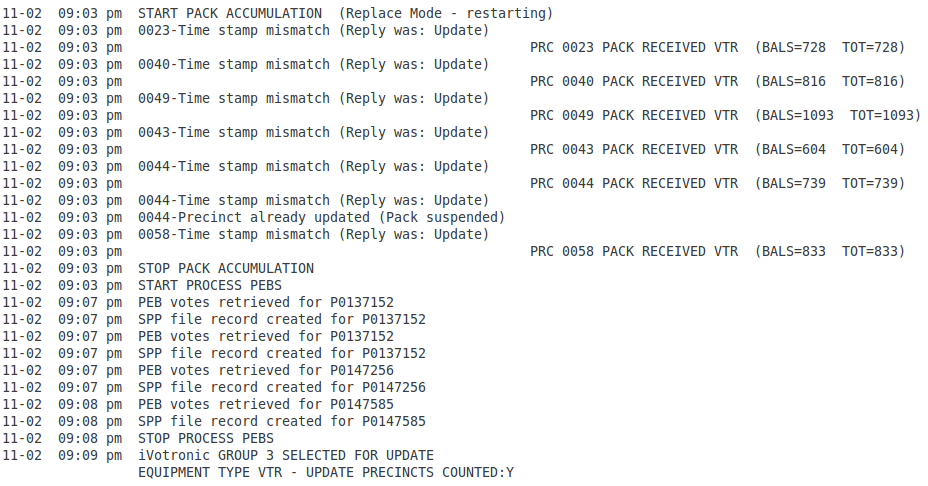
\includegraphics[width=0.9\textwidth]{system}
%This is app~\ref{app:sl}
\end{center}


\end{document}
